\documentclass[12pt,a4paper,twoside,openright]{report}
\usepackage{algpseudocode}		% ambienti per la scrittura di algoritmi
\usepackage{algorithm}			% 

\usepackage{epsfig}						% figure eps
\usepackage{graphicx}					% figure qualsiasi
\usepackage{amsmath,amsfonts,amsthm}		% package di scrittura matematica
\usepackage{amssymb}
\usepackage{psfrag}
\usepackage{fancyhdr}
\usepackage{u

\end\documentclass{beamer}

% \usepackage{beamerthemesplit} // Activate for custom appearance

\title{Example Presentation Created with the Beamer Package}
\author{Till Tantau}
\date{\today}

\begin{document}

\frame{\titlepage}

\section[Outline]{}
\frame{\tableofcontents}

\section{Introduction}
\subsection{Overview of the Beamer Class}
\frame
{
  \frametitle{Features of the Beamer Class}

  \begin{itemize}
  \item<1-> Normal LaTeX class.
  \item<2-> Easy overlays.
  \item<3-> No external programs needed.      
  \end{itemize}
}2
\end{document}
\begin{figure}[htbp] %  figure placement: here, top, bottom, or page
   \centering
   \includegraphics[width=2in]{example.jpg} 
   \caption{example caption}
   \label{fig:example}
\end{figure}\documentclass[11pt, oneside]{article}   	% use "amsart" instead of "article" for AMSLaTeX format
\usepackage{geometry}                		% See geometry.pdf to learn the layout options. There are lots.
\geometry{letterpaper}                   		% ... or a4paper or a5paper or ... 
%\geometry{landscape}                		% Activate for for rotated page geometry
%\usepackage[parfill]{parskip}    		% Activate to begin paragraphs with an empty line rather than an indent
\usepackage{graphicx}				% Use pdf, png, jpg, or eps§ with pdflatex; use eps in DVI mode
								% TeX will automatically convert eps --> pdf in pdflatex		
\usepackage{amssymb}

\title{Brief Article}
\author{The Author}
%\date{}							% Activate to display a given date or no date

\begin{document}
\maketitle
%\section{}
%\subsection{}



\end{document}  % XeLaTeX can use any Mac OS X font. See the setromanfont command below.
% Input to XeLaTeX is full Unicode, so Unicode characters can be typed directly into the source.

% The next lines tell TeXShop to typeset with xelatex, and to open and save the source with Unicode encoding.

%!TEX TS-program = xelatex
%!TEX encoding = UTF-8 Unicode

\documentclass[12pt]{article}
\usepackage{geometry}                % See geometry.pdf to learn the layout options. There are lots.
\geometry{letterpaper}                   % ... or a4paper or a5paper or ... 
%\geometry{landscape}                % Activate for for rotated page geometry
%\usepackage[parfill]{parskip}    % Activate to begin paragraphs with an empty line rather than an indent
\usepackage{graphicx}
\usepackage{amssymb}

% Will Robertson's fontspec.sty can be used to simplify font choices.
% To experiment, open /Applications/Font Book to examine the fonts provided on Mac OS X,
% and change "Hoefler Text" to any of these choices.

\usepackage{fontspec,xltxtra,xunicode}
\defaultfontfeatures{Mapping=tex-text}
\setromanfont[Mapping=tex-text]{Hoefler Text}
\setsansfont[Scale=MatchLowercase,Mapping=tex-text]{Gill Sans}
\setmonofont[Scale=MatchLowercase]{Andale Mono}

\title{Brief Article}
\author{The Author}
%\date{}                                           % Activate to display a given date or no date

\begin{document}
\maketitle

% For many users, the previous commands will be enough.
% If you want to directly input Unicode, add an Input Menu or Keyboard to the menu bar 
% using the International Panel in System Preferences.
% Unicode must be typeset using a font containing the appropriate characters.
% Remove the comment signs below for examples.

% \newfontfamily{\A}{Geeza Pro}
% \newfontfamily{\H}[Scale=0.9]{Lucida Grande}
% \newfontfamily{\J}[Scale=0.85]{Osaka}

% Here are some multilingual Unicode fonts: this is Arabic text: {\A ?????? ?????}, this is Hebrew: {\H ????}, 
% and here's some Japanese: {\J ???}.



\end{document}  

\endrl}
\usepackage{array}
\usepackage{subfigure}
\usepackage{lscape}
\usepackage{colortbl}
\usepackage{alltt}
\usepackage{tabularx}
\usepackage[english]{babel}
\usepackage[nottoc]{tocbibind}
\sloppy
\raggedbottom

\linespread{1.3}
\renewcommand{\baselinestretch}{1.3}

\makeatletter
\def\cleardoublepage{\clearpage\if@twoside \ifodd\c@page\else
\hbox{}
\vspace*{\fill}
\begin{center}
%This page intentionally contains only this sentence.
\end{center}
\vspace{\fill}
\thispagestyle{empty}
\newpage
\if@twocolumn\hbox{}\newpage\fi\fi\fi}
\makeatother

%\newcites{wb}{Web References}

%------------------------------------------------------
% Impostazioni per il controllo sillabazione vedove/orfane ect..
%
% \looseness=1 o \looseness=-1 prima di un paragrafo per
% allungarlo o accorciarlo di una riga
%------------------------------------------------------

\lefthyphenmin=4
\righthyphenmin=4
\tolerance=1000
\hyphenpenalty=100
\emergencystretch=1 cm

\widowpenalty=5000
\clubpenalty=2500

%--------------------------------------------------------
% impostazioni per la dimensione delle pagine
%--------------------------------------------------------
\renewcommand{\headrulewidth}{0.5pt}
\hoffset=-15mm
%\topmargin=0mm
\headheight=15pt
\textwidth=140mm
\headsep=5mm
\voffset=-5mm
%\hsize=13cm
%\textwidth=164mm
\textheight=230mm
\evensidemargin=25mm
\oddsidemargin=25mm
%\marginparwidth=0mm

\renewcommand{\abovecaptionskip}{0pt}
\renewcommand{\belowcaptionskip}{0pt}

%--------------------------------------------------------------
%impostazione headers
%--------------------------------------------------------------
\pagestyle{fancy}
%\addtolength{\headwidth}{\marginparsep}
%\addtolength{\headwidth}{\marginparwidth}
\renewcommand{\chaptermark}[1]{\markboth{#1}{}}
\renewcommand{\sectionmark}[1]{\markright{\thesection\ #1}}
\fancyhf{}
\fancyfoot[LE,RO]{\bfseries\thepage}
\fancyhead[RO]{\bfseries\rightmark}
\fancyhead[LE]{\bfseries\leftmark}
\fancypagestyle{plain}{%
\fancyhead{} % get rid of headers
\fancyfoot{}
\renewcommand{\headrulewidth}{0pt} % and the line
}

\newenvironment{myverse}
{\small}
{}

\newenvironment{myabstract}{%
  \begin{center}%
    \null\vfil
    \bfseries \abstractname
  \end{center}}%
{\par\vfil\null}

%------------------------------------
\newcommand{\name}{$\mathcal{H}$eaven } 
\newcommand{\namens}{$\mathcal{H}$eaven} 
%------------------------------------
\begin{document}

\pagenumbering{roman}
\setcounter{page}{1}
\pagestyle{empty}

%--------------------------------------------------------------------------------
% include title page
%--------------------------------------------------------------------------------
%\linespread{1}
\begin{titlepage}
\vspace*{-2.5cm}
\bfseries
\begin{center}
  \LARGE
  Politecnico di Milano\\
  \Large
  Facolt\`{a} di Ingegneria dell'Informazione\\


\psfig{file=images/logopm,width=4cm}

\begin{large}
Corso di Laurea Magistrale in Ingegneria Informatica\\
Dipartimento di Elettronica, Informazione e Bioingegneria\\
\end{large}

\vspace{1.0cm}
\begin{Large}
\dots Titolo della tesi \dots\\
\dots al massimo su due righe \dots
\end{Large}  
\end{center}
\vspace*{5.5cm}
\large
\begin{flushleft}
\hspace{-2cm}  Advisor: Emanuele DELLA VALLE\\
\hspace{-2cm}  Co-Advisor: Daniele DELL'AGLIO\\
\end{flushleft}
\vspace*{1.5cm}

\hspace{1.5cm}
\parbox{14cm}{
    \begin{tabular}{lll}
        Master thesis by: & Riccardo TOMMASINI     & matr. 799120\\
    \end{tabular}
}

\vspace*{1.4cm}
\begin{center}

  Academic Year 2013-2014



\end{center}
\end{titlepage}
\cleardoublepage

%--------------------------------------------------------------------------------
% dedica
%--------------------------------------------------------------------------------
\thispagestyle{empty}

\begin{flushright}
\Large\textit{dedica\dots}
\end{flushright}

%\null\vfil

\cleardoublepage

%--------------------------------------------------------------------------------
% ringraziamenti
%--------------------------------------------------------------------------------
\thispagestyle{empty}

\chapter*{Thanks To}
Ringraziamenti vari, massimo una o due pagine.

\begin{flushleft}
Milano, 1 Aprile 2005
\end{flushleft}

\begin{flushright}
\emph{\dots Fabio \dots}
\end{flushright}

\cleardoublepage
\thispagestyle{empty}

\pagestyle{fancy}
\renewcommand{\contentsname}{Table of Contents}%

%--------------------------------------------------------------------------------
% include the abstract in italian
%--------------------------------------------------------------------------------
\chapter*{Estratto}
Lo Stream Reasoning \`e  il settore di ricerca che ha dimostrato la possiblit\`a di applicare procedure di reasoning su flussi informativi in rapido cambiamento. Un RDF Stream Processing (RSP) Engine \`e  un sistema in grado di processare a livello semantico questi flussi, quando sono codificati secondo lo standard RDF. Il numero di RSP Engine implementati \`e  in crescita e di conseguenza la comunit\`a scientifica sta formalizzando i metodi e gli strumenti che hanno consentito lo sviluppo di queste soluzioni.

Diversi settori di ricerca nell'ambito della Computer Science, hanno mostrato interesse per una maggiore comprensione della natura del proprio lavoro. Sono stati fatti diversi studi che hanno analizzato i frutti della ricerca in questi settori~\cite{Tichy:1995:EEC:209090.209093, Wainer:2009:EEC:1518331.1518552}. Questi hanno dimostrato anzitutto la natura ingegneristica di molte pubblicazioni nell'ambito della Computer Science, ma anche una discreta mancanza di valutazioni empiriche delle soluzioni implementate. Questa \`e  una differenza evidente con le altre aree di ricerca legate al mondo dell'ingegneria, che si focalizzano su questo tipo di analisi.

Solitamente, nei settori informatici in cui la valuazione empirica \`e tralasciata, i sistemi proposti hanno una natura complessa e sfaccettata che \`e difficile da valutare. Tuttavia \`e  possibile, con gli strumenti adatti, studiare anche casi complessi. Questo accade per le scienze sociali o l'economia, i cui soggetti d'indagine non sono di certo facilmente modellabili. In questi settori viene comunemente usato un approccio comparativo sistematico, che semplifica il problema di affrontare soggetti complessi, senza tralasciare gli aspetti che li rendono rilevanti. Questo approccio diventa applicabile solo in un contesto sperimentale appropriato, che garantisce propriet\`a come riproducibilit\`a, ripetibilt\`a e comparabilit\`a.

La comunit\`a dello Stream Reasoning ha colto la necessit\`a di fornire strumenti per valuare correttaemente gli RSP Engine,  comprenderne il comportamento e quantificarne il valore comparando le prestazioni in casi d'uso reali. Qualche passo in questa direzione \`e  stato gi\`a fatto. Lavori recenti~\cite{Zhang2012, LePhuoc2012c, DBLP:conf/semweb/DellAglioCBCV13} hanno fornito framework di benchmarking per RSP Engine, mentre altri hanno posto le basi di queste valutazioni~\cite{DBLP:conf/esws/ScharrenbachUMVB13}, mostrando quali erano le mancanze di tali framework.

Le soluzioni proposte si sono dimostrate limitate, e la valutazione empirica di RSP Engine \`e  solo all'inizio. Quello che ancora manca \`e  una infrastruttura che permetta la comparazione sistematica di RSP Engine, all'interno di un contesto sperimentale che goda delle proprit\`a sopracitate. Per affrontare il problema, in questa tesi, abbiamo preso dall'ingegneria aerospaziale l'idea di un banco di prova, uno strumento di valutatione e sviluppo per motori.

Un banco di prova permette di progettare esperimenti ed eseguirli su qualsiasi motore, raccogliendo i dati per una successiva valutazione delle prestazioni. %Dal punto di vista scientifico un esperimento gode di tre proprit\`a fondamnetali: riproducibilit\`a, ripetibilit\`a e comparabilit\`a, tre pilastri su cui \`e  possible costrurie un approccio comparativo sistematico per la ricerca. 
La nostra domanda di ricerca quindi \`e : "Un banco di lavoro per RSP Engine \`e  la soluzione che permetta la ricerca comparativa e sistematica nell'ambito dello Stream Reasoning?"

In questa tesi proponiamo \namens, un framework open source per la ricerca comparativa e sistematica nell'ambito dello Stream Reasoning. Il framework si compone di un Banco di Lavoro, l'equivalente di quanto abbiamo visto nell'ingegneria aerospaziale ma per RSP Engine. Include quattro implementazioni naive di RSP Engine, dette Baselines. Questi sistemi semplificati permettono di iniziare la ricerca comparativa. Infine \name contiene l'Analyser, un insieme di metodi di indagine e strumenti di supporto, organizzati gerarchicamente ed atti ad analizzare e comparare i dati raccolti attraverso l'esecuzione di esperimenti su RSP Engine tramite il banco di lavoro.


%--------------------------------------------------------------------------------
% include the abstract in english
%--------------------------------------------------------------------------------
\chapter*{Abstract}
Stream Reasoning research field is grown enough to prove that reasoning upon rapidly changing information is possible. The number of implemented RDF Stream Processing (RSP) Engine, systems capable to handle at semantic level RDF-encoded information flows, is increasing. Now the Stream Reasoning community is working on the standardisation of the methods and tools that supported the development of those solutions. Moreover, it is mandatory to provide an evaluation of RSP Engines, which allows to understand how these systems perform in real uses cases. 
Recent works in the filed \cite{Zhang2012, LePhuoc2012c, DBLP:conf/semweb/DellAglioCBCV13} pursued this goal, providing many benchmarks for evaluating RSP Engines. Further analysis of RSP Engines \cite{DBLP:conf/esws/ScharrenbachUMVB13} pointed out the challenges involved by the Stream Reasoning research. \cite{DBLP:conf/esws/ScharrenbachUMVB13} posed the basis for a proper evaluation of such a system, describing in detail where these works have failed and where the can be improved.

In parallel, many  Computer Science (CS) research fields tried to understand the nature of their own research. The related studies \cite{Tichy:1995:EEC:209090.209093, Wainer:2009:EEC:1518331.1518552} shown the affinity of many CS research fields to an Engineering epistemology. But they also evinced and criticised the concrete differences with other engineering research areas, which focus on evaluation of the proposed systems and not only on their design and development. The lacks of an empirical approach can be ascribed to the complex nature of the software systems. However, it is possible to face complex case studies which are not be easily modelled. Social science and economy researchers found methods to deal with them.

The Stream Reasoning research suffers from the same lack. The limitations of the existing benchmarking proposals proved that the empirical evaluation of RSP Engines is just at the beginning. What is still missing in an infrastructure that allows to compare, maybe automatically, the performances of many RSP Engines. We borrow from the aerospace engineering the idea of an engine test stand, which is an automatic facility for engine testing. A test stand allows to design experiments and to execute them, evaluating engines in a controlled environment. %Experiment properties like reproducibility, repeatability and comparability represent the pillars upon which we can start the empirical evaluation of RSP Engines.
Thus, we formulate the following research question: "\textit{Can an engine test stand, together with queries, datasets and methods, support Systematic Comparative Research Approach for Stream Reasoning?}"

In this thesis we propose \namens, an open source framework that enables the Systematic Comparative Approach in the Stream Reasoning research field. \name consists in:  an RSP Engine Test Stand, which emulates the aerospace engineering facility in the Stream Reasoning context; the Analyser, which enables the Systematic Comparative Approach trough a set of methods and tools for the investigation, hierarchically organised into an stack; and, finally, four naive implementations of RSP Engines, called Baselines, which represent simple terms of comparison upon which  start the comparative research.

%--------------------------------------------------------------------------------
% talbe of contents
%--------------------------------------------------------------------------------
\tableofcontents
\cleardoublepage

\pagenumbering{arabic}

\setcounter{page}{1}


%--------------------------------------------------------------------------------
% introduction
%--------------------------------------------------------------------------------
\chapter{Introduction}
\label{chap:introduction}
\section{Contributions}
\subsection{Heaven}
\subsection{RSPEngine inside DSMS}
\subsection{Experiments}

\section{Structure of this Thesis}

Blablabla

Esempio di figura

\begin{figure}[ht]
%\centerline{\epsfig{file=esempio.ps, width=12 true cm}}
\caption{Didascalia esempio di figura.}
\label{fig:esempio}
\end{figure}

Esempio di equazione

\begin{equation}
\dot V_4= - k_v \lambda (z_1- \varepsilon \lambda z_3)^T(z_1-
\varepsilon \lambda z_3).
\end{equation}


\chapter{Background}
\label{chap:background}
\section{Semantic Web}
\section{Stream Processing}
\section{Stream Reasoning}
\section{Empirical Research}

Tichy and collaborators [15] evaluated 400 articles published in 1993, 50 of them randomly selected papers published by ACM in 1993 and the rest systematically selected from a few journals in Systems and Software Engineering, and classified the research re- ported in the paper in five categories (quoting [15] definitions): \begin{itemize}
\item Formal theory: articles whose main contributions are formally tractable propositions, e.g., lemmata and theorems and their proofs.
\item Design and modelling: systems, techniques, or models, whose claimed properties cannot be proven formally. Examples include software tools, performance prediction models, and complex hardware and software systems of all kinds. The papers in this class were further classified in the categories 0\%, 0–10\%, 10– 20\%, 20–50\, and +50\%, according to the proportion of the paper that was dedicated to the evaluation of the new system, technique, or model.
\item Empirical work: articles that collect, analyse, and interpret observations about known designs, systems, or models, or about abstract theories or subjects (as this paper does). The emphasis is on evaluation, not on new designs or models.
\item Hypothesis testing: articles that define hypotheses and describe experiments to test them.
\item Others: articles that do not fit any of the four categories above, e.g., surveys.
\end{itemize}

\subsection{Software Testing}
\subsubsection{SOAK}
\subsubsection{Stress}

\section{Benchmarks}
\subsection{TCP}  \label{sec:tcp}


\subsection{Reasoning Benchmark}
\subsubsection{LUBM}
\subsection{DBMS \& CEP Benchmarking}
\subsubsection{Linear Road}
\subsection{Stream Reasoning Benchmark}
\subsubsection{SRBench}
SRBench [5] proposes a suite of test queries and defines metrics to evaluate the
performance of the system. This benchmark contains 17 queries to gather the
properties of the RDF stream engines. The queries vary to ensure that several
features of the target system are tested: queries involving single or multiple input
streams, queries over stream-only data sources or over mixed stream and static
data source, etc. In [5] the authors applied the benchmark on the existent RDF
stream engines, and explained the differences in term of supported functionalities.
Time and memory performance tests, and scalability tests are not targeted
in the actual version of SRBench.
\subsubsection{LSBench}
LSBench [6] proposes three tests to evaluate the RDF stream engines. The
first one is a functional test to verify the operators and the functionalities supported
by the engines: it is a test similar to the one proposed by SRBench. The
second test is a correctness test: its goal is to verify if the tested RDF stream
engine produces the correct output. Actually this analyses only the number of
produced answers, assuming that the contents of the output are correct. Finally,
the third test is a maximum input throughput test: it has the goal evaluate the
maximum throughput of the RDF stream engines. This test is done increasing
the rate of data in the stream and verifying the number of the answers. For each
test a set of 12 queries is provided; similarly to SRBench, the queries vary to
take into account different features of the engines (single and multiple streams,
presence of static data, etc)

\subsubsection{Correttezza}
\subsubsection{Seven Commandaments}



%--------------------------------------------------------------------------------
% problem settings
%--------------------------------------------------------------------------------
\chapter{Problem Settings}
\label{chap:problem-settings}
In this Chapter we introduce the work this thesis involved. First we introduce the motivations behind this research. In Section \ref{sec:comparative-research} we describe the themes that have inspired this survey towards the Comparative Research and, as a conclusion, we formulate our research question. Then, in Section \ref{sec:requirements} we formalise the requirements we have to satisfy in order to successfully answer the research question.

\section{Comparative Research}\label{sec:comparative-research}
The Computer Science (CS) community classifies its activity in many works and shows that its research mostly follow an engineering epistemology \cite{Wainer:2009:EEC:1518331.1518552,Tichy:1995:EEC:209090.209093}. A majority of publications belongs to \textit{empirical work} and \textit{design \& modelling} classes of Tichy's taxonomy (See \ref{sec:tcp} ) and, among them, proposals of new systems or models  are more common then the evaluations of existing ones. This contrasts with other engineering areas, where the experimental research is almost dominant. CS needs to focus on collecting, analysing, and interpreting the observations of those works it usually only designs or implements. Now the question is: \textit{What are the motivation under this CS research lack?} The main problem in evaluating software systems or models regards their complex and multifaceted nature. Other explanations concern the difficulties of conducting realistic evaluations, because of the number of the involved variables.

A Systematic Comparative Research Approach (SCRA) is typically used in those research fields where the complexity of its research subjects goes beyond the possible observable models. This is the case of the social sciences, which exploit techniques to deal with complex cases that can not be simplified in experimental setting. The analysis of a single case study allows to deeply understand it, but it makes difficult to engage any form of generalisation. On the other hand, cross-case studies are more relevant and allow general thinking, but their final complexity represents a problem. We need a strategy that reduces the analysis complexity without lose the relevance of each involved system. In this regard, Russel Schutt discusses four stages to systematic qualitative comparative studies for history social phenomena:
\begin{enumerate}
\item[S.1] Premise of the investigation: identification of possible causes.
\item[S.2] Choose the cases to examine (location, language, gender).
\item[S.3] Examine the similarities and the differences with shared methods.
\item[S.4] Propose a causal explanation for the phenomena.
\end{enumerate} We will return on these stages later. Is important to understand that this investigation method becomes meaningful inside the experimental environment. An \textit{experiment} is a test under controlled conditions that is made to demonstrate a known truth or examine the validity of an hypothesis (W.R Inge). Complex cases are seen as a combination of known properties upon which is possible to identify parallelism or state contrasts and are used to set up experiment configuration. Researcher can exploit the notions of \textit{reproducibility} to appreciate variations on changing experiment conditions, \textit{repeatability} to consolidate observations trough multiple identical executions and \textit{comparability} to contrast the results to identify the differences.

Some Computer Science sub-fields attempt to lead Case-driven analysis by the notion of experiment. Database community explores the idea of comparative research trough benchmarking techniques and actually the quality of empirical studies is rising \cite{Wainer:2009:EEC:1518331.1518552}. It is worth to note Jim Gray's work about transactional benchmarking (TCP, Section \ref{sec:tcp}) and Domain Specific Benchmarks (DSB). He states that \textit{any comparison on performances starts with the definition of a benchmark or a workload}, but we need know the relevance of the metrics. Measurement variations are very frequent from one application to another, because each system is thought to solve a small problems set. A DSB must response properly to system diversities, by specifying a synthetic workload to describe typical applications in the problem domain; moreover it must provide workload performances on various systems and an estimation of relative performance on the problem domain.
Gray proposes also four criteria that a DSB must meet, which are:
\begin{enumerate}
\item[G.1] \textsc{Relevance}, it must measure the performance peak of systems when
performing domain typical operations.
\item[G.2] \textsc{Portability}, it must be easy-to-implement on many different systems and architectures
\item[G.3] \textsc{Scalability}, it must be meaningful for both small and large computer systems
\item[G.4] \textsc{Simplicity}, it must be understandable to obtain credibility
\end{enumerate} 

Let's consider the relation between this criteria and Schutt's stages presented above. Gray states G.1 to identify the relevant metrics for the evaluation, as Schutt does in his first stage (S.1), which demands a pre-analysis phase of the phenomenon. Moreover, Social Science does not care about problem scaling, because those properties that define the case also determine the problem dimension (S.2). Gray poses the same concept in the DB context with G.2, demanding implementation-related conditions, but it also explicit the need to consider the dimension-related issues in G.3, because DB must consider the scaling problem. Last but not least, G.4 demands simplicity to obtain credibility while S.3 suggests to exploit those evaluation methods that are commonly accepted (shared) by the research community. 

Motivated by the growing number of RDF Stream Processing techniques, the Stream Reasoning (SR) community strongly calls of evaluation practices to allow comparison on them. RSP Engines, the systems that implement this techniques, have an high resulting complexity (Further details in Section \ref{sec:sfp}). The execution mechanism they implement together with their execution semantic and the environment where this execution happens are evaluation-related characteristics, which demonstrate that a meaningful comparison between RSP Engines is non-trivial. Chapter 	\ref{chap:evaluation} shows in details that may be difficult to analyse those system, even in case of simple and well defined architectures. 
The interest on cross-case analysis between complex subjects draw the need of a comparative research approach. Initial efforts in this direction try to define frameworks that resume  DSMSs \cite{arasu2004linear} and Reasoning \cite{Guo2005} benchmarking studies. LS Bench and SR Bench propose a set of queries, data sets, and methods to test and compare existing RSP engines (see Section\ref{sec:sr-benchmarking}). Both these works share a common background: the Linear Road Benchmark (LRB) is the only existing benchmark for relational data stream processing engines. Actually LRB only states which requirements a benchmarked DSMS must satisfy, without proposing a concrete solution. LS Bench and SR Bench implement and extend this work, but they do not re-contextualise this requirements in SR context. Following discussions identify other lacks, i.e none of them completely face the problem of evaluating query result correctness, because they do not analyse engine semantics. LS Bench concentrates attention to the evaluation of engines throughput and it checks the correctness of the query result measuring the mismatch after comparing different RSP Engines. SR Bench entirely ignores this issue and analyses the coverage of SPARQL constructs for each commercial engine. More recent works describe deeply all the RSP Engine properties, identify the future challenges and provide a standardization benchmarking requirements: commandments for a meaningful testing on RSP Engines\cite{DBLP:conf/esws/ScharrenbachUMVB13}.

Stream Reasoning community still lacks an infrastructure that can control the execution environment and allow to systematic testing. LRB provides a simulator to validate the benchmarked DSMS systems, but does not face the problem of an online evaluation it. Researches in this area demonstrates that RSPEngine execution semantic is relevant \cite{Botan:2010:SMA:1920841.1920874}, but does not evaluate its cost. From the aerospace engineering we borrow the idea of an \textit{Engine Test Stand}, a tool that allows experiments design, their systematic execution and automatic results comparison. An engine can not be evaluated only by an architectural viewpoint, it is necessary to understand it behaviour during the execution: \textit{A process cannot be understood by stopping it. Understanding must move with the flow of the process, must join it and flow with it}\footnote{The First Law of Mentat, quoted by Paul Atreides to Reverend Mother Gaius Helen Mohiam}. Thus, the community questioned itself \textit{How to support SRCA on RSP Engines}? Now we have queries, dataset and methods, that partially answer it and the new research question is "\textit{Can an engine test stand, together with queries, datasets and methods, support SCRA for Stream Reasoning?}". The next section poses the requirements a proper answer to this research question must satisfy.

\section{Requirements} \label{sec:requirements}

In order to simplify and support Systematic Comparative Research Approach on RSP engines trough an Engine Test Stand we need to answer the following questions: 
\begin{enumerate}
\item[Q.1] How can the behaviour of system be evaluated? 
\item[Q.2] What makes this evaluation rigorous? 
\item[Q.3] How can this rigorous evaluation be automated?
\end{enumerate} To answer Question Q.1 we exploit traditional definition of \textit{experiment} presented above. We answer Q.2 referring to \textit{reproducibility}, \textit{repeatability}, and \textit{comparability} of experiments. Trough this concepts it is easy to answer Q.3 formalising the requirements for the solution.

\textit{Reproducibility} refers to measurement variations on a subject under changing conditions. We gather this conditions into experiment configuration, whose specification is up to the user. For this reason the solution must be independent from:
\begin{enumerate}
\item[R.1] \textit{Test data}, relevant RDF data streams and ontologies chosen from user domain of interest. %R.2.1
\item[R.2] \textit{Query}, relevant queries registered from user domain of interest.
%thus allowing users to register relevant queries from their domains of interest. %R.2.2
\item[R.3] \textit{Engine}, any RSP Engine tested by the means of easy-to-implement software interfaces. 
%thus allowing users to put an RSP engine on the test stand by the means of easy to implement software interfaces, e.g., it should adopt an event-base architecture as normally done by RSP engines and present events to RSP engine in a simple to parse RDF serialisation. %R4 e R5
\end{enumerate}

\textit{Repeatability} refers to variations on repeated measurements on a subject under identical conditions. The solution must not affect the RSP engine evaluation, which, from a practical point of view, poses two requirements:
\begin{enumerate}
\item[R.4] it must not be running when the RSP engine is under execution. %R.1.2
\item[R.5] it must have reduced (and possibly constant) memory footprint. %R.1.1
\end{enumerate}

\textit{Comparability} refers to performance measurements nature and the relations between experimental conditions. The SCRA demands both the definition of \textit{comparable metrics} and the standardization of \textit{evaluation methods}, which means the solution must:
\begin{enumerate}
\item[R.6] include \textit{basic set of performance measurements} \cite{DBLP:conf/esws/ScharrenbachUMVB13}.
\item[R.7] enable users extensions with new software sensors and specific measurements collection.
%\item[R.7] enable users software extensionsa and specific measurements collection.
\item[R.8] support performance measurements collection for further analysis.
\item[R.9] allow \textit{qualitative analysis} trough tools for result visualization
\end{enumerate}


In terms of software engineering, any solution which satisfies the requirements above demands also some technical ones: 
\begin{enumerate}
\item[R.10] \textit{Extendible Design}, the possibility to replace theoretically each module with one with the same interfaces, but different behaviour, without affecting architecture stability.
\item[R.11] \textit{Event-base architecture} to properly communicate with  RSP Engines, which normally exploit it.
\item[R.12] \textit{Easy-to-Parse RDF Serialisation} for the events presented to the RSP Engine in exam
\end{enumerate}

SCRA is case-oriented, it needs \textit{successful analysis and evaluations examples} to pose experimental guidelines and \textit{initial terms of comparison}. We call baseline an elementary solution for the RSP problem, which is relevant from an experimental viewpoint. To fulfil this request the answer to our research question must consider to have specific baseline modules and satisfy their own requirements, which are: \begin{enumerate}
%\item[R.13] Be a Solution: it solves the problem entirely, without concerning about performance. % devono risolvere interamente il problema, nel nostro caso devono essere complete e sound rispetto ad entailment regime che si è scelto
\item[R.13] It must be Elementary: requiring the minimum design effort, which means be a naive solution and do not care about performances.  % non devono essere soluzioni smart, devono chiedere il minimo effort
\item[R.14] It must be Eligible: being a fair term of comparison w.r.t. commercial solutions. %e' inutile se sono sopra un'ordine di grandezzaad esempio in latenza, rispetto ad una soluzione commerciale. probabilmente è sbagliata la domanda di ricerca
\item[R.15] It must be Relevant: covering one of the theoretical solutions. %la soluzione che coprono deve essere una delle immediate soluzioni del problema iniziale: Graph vs Statement o Inc vs Naive, tempo controllato esternamente, ecc
\item[R.16] It must be Simple: allowing to identify easily those characteristics which support hypothesis formulation and comparison.  %non devono offrire api più complesse rispetto a un RSPEngine tradizion	ale.
\end{enumerate}

%Some of those requirements assume a problem-specific meaning. As advocated in the early works on Stream Reasoning \cite{1,2} the most simple approach to create a stream reasoning system is arrange into a pipeline DSMS with a reasoner. Baselines design must follow this statement to develop a full solution [R.13] which is very simple w.r.t the commercial ones presented in Chapter 2 [R.14]. Chapter 2 also states how two main design decisions can distinguish the baselines: the RDF stream model and the architecture. From this point of view the solution must provide at least four Baselines [R.16], which cover all possible combinations those design choices.


%--------------------------------------------------------------------------------
% heaven
%--------------------------------------------------------------------------------

\chapter{Heaven - Design}
\label{chap:heaven}
In this chapter we present  \namens,  an open source framework for Systematic Comparative Research on RSP Engine.
It consists in four baselines and two main components: the Test Stand and the Analyser. Firstly, Section \ref{sec:teststand} introduces the Test Stand, which satisfies requirements from R.1 to R.8 and from R.10 to R.12, by executing experiments on an RSP Engine. Section \ref{sec:baselines} describes the Baselines, four RSP Engines that are included in \name as naive terms of comparison, since they fulfil requirements R.13 and R.14. Finally, Section \ref{sec:analyser} presents the Analyser, which addresses requirements R.9 and R.10  allowing the user to visualise, investigate and compare experiment results. %Soundness and completes of the query answering process are assessed post-hoc by comparing the results of an RSP engine with a term of comparison whose results are correct (see Section 5).

\section{Test Stand}\label{sec:teststand}

Aerospace engineering defines an engine test stand as a facility used to develop, study and characterise engines. It allows to test operating regimes and offers measurement of several variables associated with engine process. A test stand may uses actuators for attaining a specific engine state, which is a unique combination of the engine properties. The information collected through the sensors depends on the engine manufacturer, which usually provides his own stand or the facilities to test the engine with commercial solutions. The test stand executes black box testing over engines, because its users can not rely to known engine internal mechanisms.

The definition above still holds its relevance in the SR context, with the difference that engines subject of the testing, RSP Engines, are IO-Systems. An RSP Engine consumes an RDF Stream and  produces a new one, by applying queries under some entailment regime and w.r.t. an ontology which does not change over time. Describing an RSP Engine means understanding the relation between input stream, the queries registered to it and what we call \textit{operational semantics}, which requires to know the RSP Engine internal processes. Indeed, black box testing is the only possibility to analyse such system with a test stand. Even having access to the entire RSP Engine code, may results hard to characterise all the RSP Engine properties a priori. 

Figure \ref{fig:architecture} shows \name \textsc{Test Stand} design. It contains the block schema of the modules that composes the \textsc{Test Stand} pipeline. Moreover, we enumerates in the Figure the events that pass trough the the \textsc{Test Stand} while it is executing and experiment. In the following subsection we describe each elements that Figure \ref{fig:architecture} summarises. In Subsection \ref{sec:modules} we describe the \textsc{Test Stand} pipeline and each module that composes it, in Subsection \ref{sec:test-stand-data-model} we detail the Data Model exploited to represent experiments, events, query results and measurements. Finally, in Subsection \ref{sec:test-stand-workflow} we describe the \textsc{Test Stand} workflow, how it executes experiments to stress the RSP Engine we want to test.

\begin{figure}[tbh]
\centering
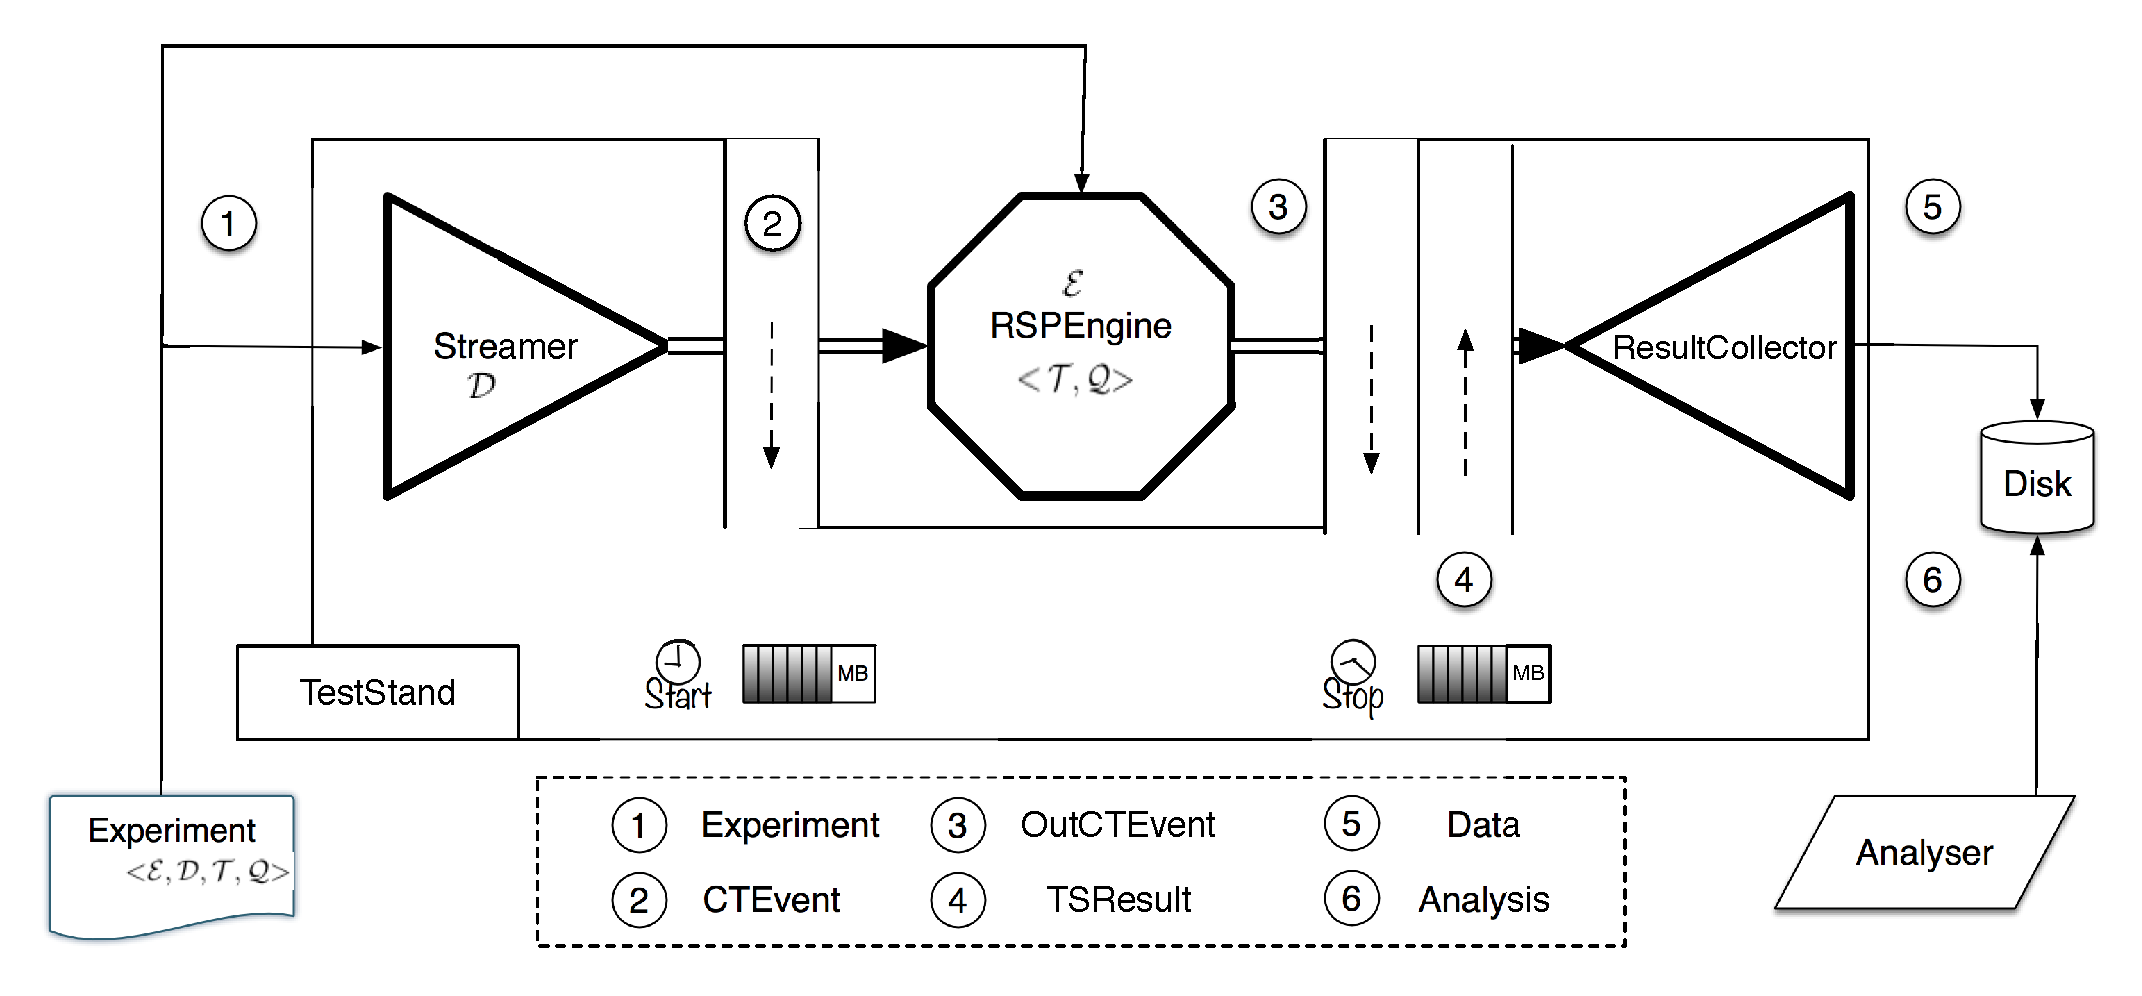
\includegraphics[scale=0.37]{images/schema2}
\caption{\name modules and workflow} 
\label{fig:architecture}
\end{figure}


\subsection{Modules}\label{sec:modules}

\noindent An aerospace test stand exploits different modules to simulate the operating regime for the engine in use ( i.e a module for fuel distribution, one for the engine mechanic support or to enable users interaction during the execution ). Modularity allows to extend the test stand and specify testing procedure. 

We design \name \textsc{Test Stand} as modular system for the same reasons, guaranteeing modularity [R.10]. Thus, it consists into the following three stand-alone modules:
\begin{itemize}
\item the \textsc{Streamer}, a source for the input RDF Stream
\item the RSP Engine we want to test;
\item the \textsc{Result Collector}, a data acquisition system for both the query results and the gathered measurements.
\end{itemize}

\noindent The architecture of \name \textsc{Test Stand} is represented in Figure \ref{fig:architecture}. The \textsc{Test Stand} modules  are arranged into a pipeline and communicates exchanging events [R.11]. Their interfaces allow each of them to be replaceable with an other ones with a different behaviour, but which complies with the interfaces specifications.

The execution starts with the \textsc{Streamer}, which hides the data generation logic in order to obtain data independence [R.1]. It pushes an RDF Stream directly to the mounted RSP Engine. It is up to the \textsc{Streamer} to respect [R.5] and not to influence the memory footprint with heavy data loading tasks. 

An interface adapts the event flow to the RSP Engine in use, fulfilling [R.2] (Engine Independence) and hiding the query registration process [R.3] (Query independence), which happens at engine level and is up to the RSP Engine provider.

The \textsc{Result Collector} is at the tail of the pipeline. It is part of the \textsc{Test Stand} because the performance measurements are processed and gathered during the execution, together with the queries results data. The \textsc{Result Collector} is responsible to save all this data at the end of each cycle, without influencing the system. The evaluation usually happens a-posteriori trough the Analyser (Section \ref{sec:analyser}). However, real time analysis of the performance measurements are possible, but they may violate some requirements like [R.4] and [R.5]. 

Last but not least, the Test Stand has an external structure that sustains other modules and can be considered as a module itself. It allows the user to control the process through accessible APIs. It gathers the data sampled by the sensors during the execution and adds them to the query results. The \textit{Test Stand} External Structure allows the user (the RSP Engine developer) to develop a specific testing procedure for a given engine. The measure set extensions are possible by adding user defined metrics, according to requirements [R.7] and [R.10]. Finally, it controls the process ensuring that the \textsc{Test Stand} does not run when the RSP Engine run as required by [R.4].

\subsection{Experiment \& Data Model}\label{sec:test-stand-data-model}

\noindent The Test Stand accepts as input an \textsc{Experiment} in the form of a tuple \\ $<\mathcal{E},\mathcal{D},\mathcal{T},\mathcal{Q},>$ where:
\begin{itemize}
\item $\mathcal{E}$ is the RSP Engine subject of the evaluation (satisfying requirement [R.3]); 
\item $\mathcal{D}$ is the input dataset [R.1]; 
\item $\mathcal{T}$ is the ontology [R.1]; 
\item $\mathcal{Q}$ is the query to be continuously answered by $\mathcal{E}$ [R.2]. 
\end{itemize}

From an experimental point of view, which metrics we sample during the execution have a different influence on the measurements. For example, asking to the system for the memory usage may influence the latency calculus or saving on disk the query results may influence the memory footprint. Thus, we define there main kinds of experiment, distinguishing on the data we want to sample and save. Notice that which experiment kind choose depends on the goal and the error tolerance of the research.

\begin{itemize}
\item Latency Experiment, where only the latency is calculated and no query result is saved on file
\item Memory Experiment, where only the memory is gathered and no query result is saved on file
\item Query Experiment, where query results are saved on file.
\item Any combination of the previous experiment types.
\end{itemize}


\noindent In order to describe the Data Model exploited by the \textsc{Test Stand}, we draw the Entity-Relation diagram in figure \ref{fig:er}. The diagram does not include entity attributes to simplify the interpretation, but they are reported in the following Logic Schema:
\begin{figure}[tbh]
  \centering
	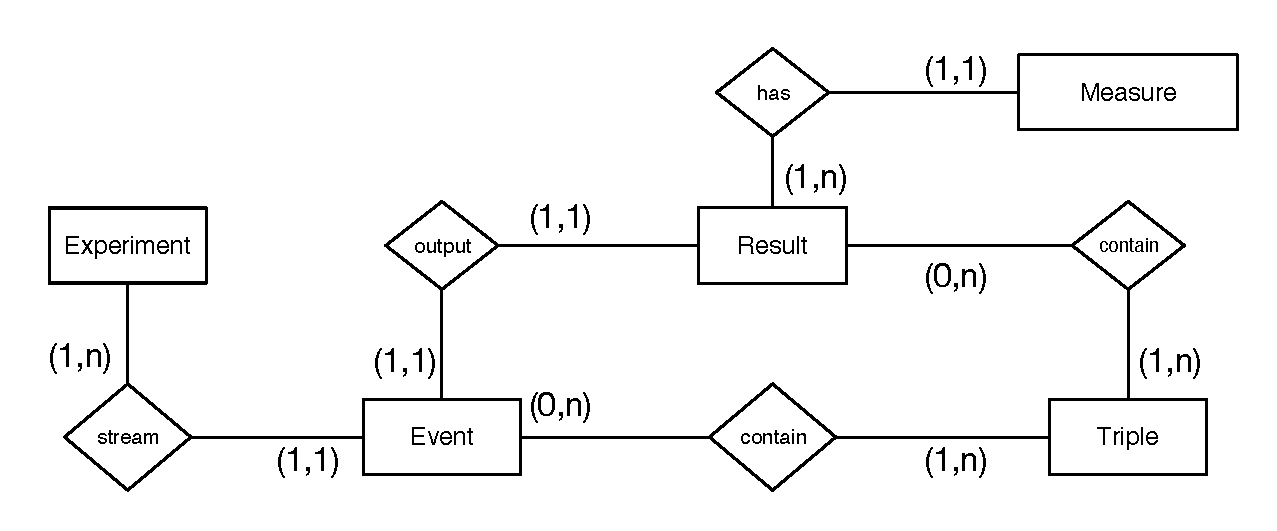
\includegraphics[width=\linewidth]{images/er-db}
	\caption{ER-Diagram \name data} 
  	\label{fig:er}
\end{figure}\\
\noindent\textsc{Experiment}(\underline{ID}, Timestamp Start, Timestamp End, Engine, Ontology, Query, Dataset, Description)\\
\textsc{Event}(\underline{ID, Experiment ID}, Timestamp)\\
\textsc{Result}(\underline{Result ID, Experiment ID}, Event ID)\\
\textsc{Measure}(\underline{ID}, Value)\\
\textsc{Measurement Set}(\underline{Measure ID, Result ID, Experiment ID})\\
\textsc{Triple}(\underline{S,P,O})\\
\textsc{Output Triple}(\underline{Result ID, Experiment ID, S, P, O})\\
\textsc{Input Triple}(\underline{Event ID, Experiment ID, S, P, O})\\

The \textsc{Experiment} entity contains the metadata of the tuple $<\mathcal{E},\mathcal{D},\mathcal{T},\mathcal{Q},>$, which semantic is explained above. "Timestamp Start" and "Timestamp End" are relevant metrics for further analysis and system control. 

The \textsc{Event} is unique inside an \textsc{Experiment}, it is possible to send two events with the same timestamp and identical tripleset. The Timestamp field allows to order events after the execution

The \textsc{Result} is associated with one and only one \textsc{Event}. It contains the results to the engine queries w.r.t the active window and the set of the measure gathered during the execution. 

The \textsc{Measurement Set} table represents the many-to-many relation between the \textsc{Result} and a number of measure that may variate  to fulfil requirement [R.7] (extendible measurement set). 

We include the concept of the \textsc{Triple} in order to model the content of \textsc{Event} and \textsc{Result}. \textsc{Input Triple} and \textsc{Output Triple} are the tables which represent two many-to-many relations, respectively between \textsc{Triple} and \textsc{Event} and \textsc{Triple}  and \textsc{Result}

\subsection{Test Stand Workflow}\label{sec:test-stand-workflow}

\noindent The \textsc{Test Stand} orchestrates the communication between the upstanding models, forcing the \textsc{Streamer} to push events to the RSP Engine and the \textsc{Result Collector} to listen the output and collect the results. To explain the \textsc{Test Stand} workflow we split the process at the points when the modules exchange events. Indeed, each message represents a different logic step in the experiment execution cycle.

Six different steps are identified by six events exchanged by \textsc{Test Stand}, \textsc{Streamer} and RSP Engine. The \textsc{Result Collector} only receives events, terminating each cycle.

In step (1) the \textsc{Test Stand} takes the experiment and starts the execution. It executes the experiment $<\mathcal{E},\mathcal{D},\mathcal{T},\mathcal{Q},>$ stressing $\mathcal{E}$ for a certain period of time looping through the steps from (2) to (5) illustrated in Figure \ref{fig:architecture}.                                                                                                                                                                                                                                                                                                                                                                                                                                                                                                                                                                                                                                                                                                                                                                                                                                                                                                                                                                                                                                                                                                                                                                                                                                                                                                                                                                                                                                                                                                                                                                                                                                                                                                                                                                                                                                                                                                                                                                                                                                                                                                                                                                                                                                                                                                                                                                                                                                                                                                                                                                                                                                                                                                                                                                                                                                                                                                                                                                                                                                                                                                                                                                                                                                                                                                                                                                                                                                                                                                                                                                                                                                                                                                                                                                                                                                                                                                                                                                                                                                                                                                                                                                                                                                                                                                                                                                                                      

In step (2), the \textsc{Streamer} pushes to $\mathcal{E}$ an event \textsc{CTEvent}. This event is a portion of an RDF Stream picked from the data $\mathcal{D}$ and it consists of a set of RDF triples with the same timestamp. In order to satisfy [R.12], it sends triple in N-Triple\footnote{\url{http://www.w3.org/2001/sw/RDFCore/ntriples/}}, which is the easiest RDF serialisation to parse.  


In step (3) $\mathcal{E}$ pushes to the \textsc{Result Collector} an event \textsc{OutCTEvent}. It contains the current answer to the query $\mathcal{Q}$ registered in $\mathcal{E}$ given the ontology $\mathcal{T}$. The \textsc{Test Stand} expects $\mathcal{E}$ to output result in N-Triple format. 

Notably, to place any RSP engine on the \textsc{Test Stand} (requirement [R.3]) \name provides a simple software wrapper that, when it receives a \textsc{CTEvent}, adapts it to the RSP engine specific format, pushes it in the RSP engine, and listens to the RSP engine output so to transform such an output in a \textsc{OutCTEvent}.

To measure performances (requirement [R.6]) the \textsc{Test Stand} performs several actions both before step (2) and after step (3) to collect data from the sensors. Previous works about Stream reasoning \cite{DBLP:conf/esws/ScharrenbachUMVB13} shows that the minimal performance measure set includes \textbf{Latency} -- defined as the delay between the injection of an event in the RSP engine and its response to it --, \textbf{Memory Load} -- defined as the difference between total system memory and the free one --, and \textbf{Completeness \& Soundness} of query-answering results. To measure latency, it starts a timer before (2) and stops it after (3). To measure memory load, it asks for the free memory of the system after step (3). Completeness \& Soundness are evaluated with post-processing analysis of the query results data.

In step (4), those observations are added to the outputs of $\mathcal{E}$ as annotations and are pushed to the \textsc{Result Collector}.  We name \textsc{TSResult} the event that contains the sensor data plus the query results produced by the engine.  

The \textsc{Test Stand} works in a single thread mode, blocking the execution of its components when it performs the measurements in (2) and (3) [R.4].  

In step (5) the \textsc{Result Collector} saves \textsc{TSResult} for post process analysis [R.9], executed trough the \textsc{Analyzer}. It does so saving the content of any TSResult  [R.8].

\section{Baselines}\label{sec:baselines}

\noindent In Chapter \ref{chap:problem-settings} we state that a Systematic Comparative Research Approach needs initial terms of comparison to lead the investigation. \name contains a set simple and easy-to-use RSP Engines called "Baselines". As the name lets to guess, these engine fulfil the four characteristics, detailed in Section \ref{sec:requirements}, required by an RSP Engine to be classified as a baseline inside the SR research field. Thus, \name Baselines are \textit{Elementary}, \textit{Relevant}, \textit{Simple} and \textit{Eligible}. developed to fulfil this lack. 

%We exploit them to define some qualitative methods of investigation and to prove the usability of the Test Stand. 
Early works on SR \cite{DBLP:conf/fis/ValleCBBC08,Walavalkar08streamingknowledge} describe the most simple approach to create a stream reasoning system: pipelining a DSMS with a reasoner. The DSMS is responsible to handle the data stream, moving from infinite sequences to finite (and processable) sets of events. The reasoner instead applies SPARQL queries on this set of events, exploiting its reasoning capabilities over a context that can be considered as static, but remains continuous. We focus on RDF Stream Processing, whose foundations, as explained in Section \ref{sec:sfp}, are: 
\begin{enumerate}
\item[1.] RDF streams, detailed in Section \ref{sec:rdfstream}
\item[2.] An extensions of SPARQL to manage continuous data (see Section \ref{sec:continuous-sparql}
\item[3.] reasoning algorithms
\end{enumerate}

\begin{figure}[tbh]
 \centering
\subfigure[Baseline A: Naive]{
	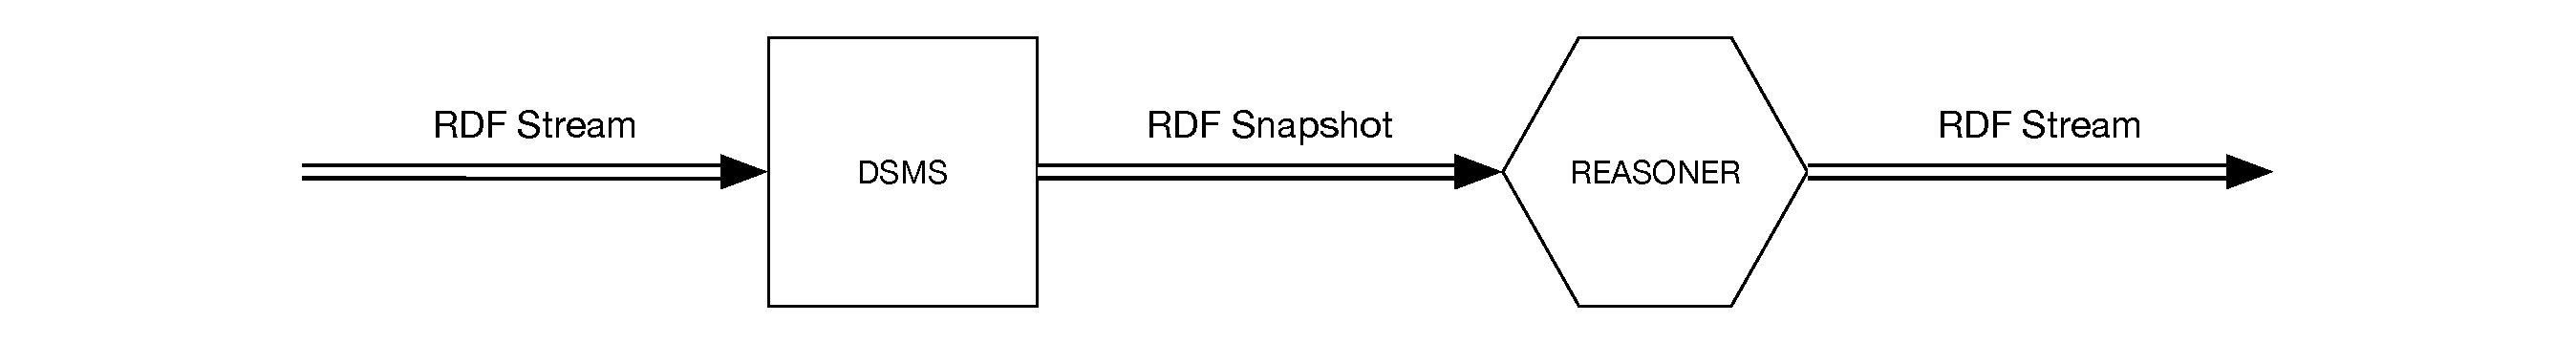
\includegraphics[width=\linewidth]{images/baseline-a}
}
\subfigure[Baseline B: Incremental]{
	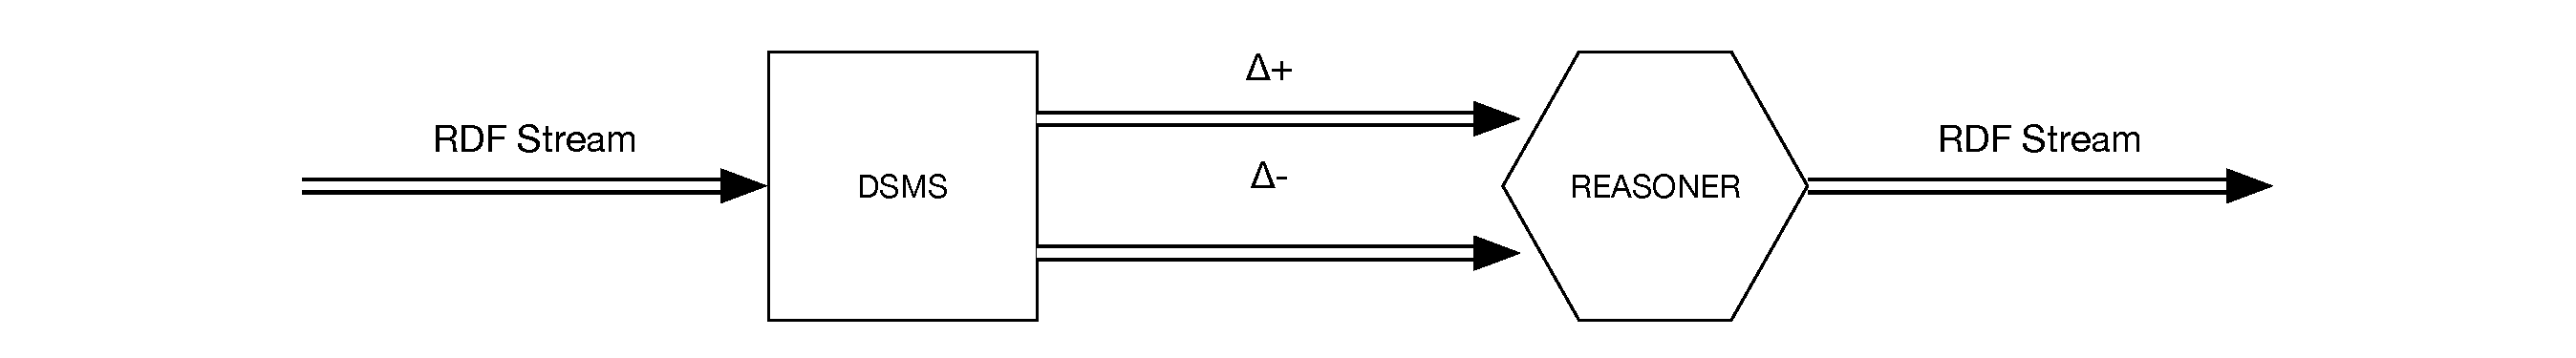
\includegraphics[width=\linewidth]{images/baseline-b}
}
	\caption{The Architecture of \name Baselines: Naive (A) and Incremental (B) Reasoning Approach}
	\label{fig:baselines}
\end{figure}

\noindent RSP Engine are those systems that can apply reasoning techniques upon rapidly changing information encoded in RDF (RDF Stream) and allow to continuous querying on the data stream (Section \ref{sec:rspengine}). It possible to develop RSP Engine following the approach described above, which actually requires to develop the integration of two existing technologies, DSMS and reasoner, and to define how they can communicate. Following we describe how this design model fulfil the requirements we posed in Section \ref{sec:requirements}.

Baselines \textit{Elementarity} can be granted by choosing a DSMS which is a reliable solution in the Information Flow Processing context and the a general purpose rule engine which is comparable with mature solutions. \textit{Elementarity} is reached when the couple elements are simple and valid terms of comparison w.r.t the state of the art.

Baselines \textit{Relevance} requires to cover all the most important theoretical variants that the "pipeline approach" conveys. In terms of reasoning we can choose between two possible approaches and with reference to the data stream processing the choices are again two. Four baseline implementations cover these two main design decisions about the RDF Stream Model and the Reasoning procedures. 

The RDF Stream model describes how the input RDF Stream is processed, different systems accept data in different models, which depends on how RDF Stream is considered in terms of events contemporaneity. The two most relevant ones are:

\begin{itemize}	
\item Triple-based model, where the events pushed in the DSMS are timestamped triples. The timestamps are non decreasing, different triples could have the same timestamp to denote that they are contemporary.
\item RDF Graphs-based: the event pushed in the DSMS are timestamped RDF graph. The timestamps are increasing and the graph is used as a form of punctuation \cite{Tatbul2003b} to separate consequent portions of the RDF stream.
\end{itemize}

The Reasoning Architecture, the techniques to make inference, depends on the way data flow from the DSMS to the reasoner. Two reasoning solutions exist for the two triples data flow:

\begin{itemize}
\item Naive solution: (Figure \ref{fig:baselines}-A) the DSMS produces an RDF Snapshot of the current windows. It sends the entire content of the window to the reasoner, which materialises all the implied triples at each cycle. This is the approach implemented in the C-SPARQL Engine \cite{DBLP:journals/sigmod/BarbieriBCVG10} and in Sparkwave \cite{DBLP:conf/debs/KomazecCF12}.
\item Incremental solution (Figure \ref{fig:baselines}-B) the DSMS outputs the IRStream, the differences between the current window and the previous one. The $\Delta^{+}$ snapshot contains the triples that have just entered in the window, while the $\Delta^{-}$ snapshot contains the triples that have just exited from the window. The reasoner, using $\Delta^{+}$ and $\Delta^{-}$, incrementally maintains the materialisation over time. This approach is taken as term of comparison in \cite{DellAglio2014} and it is inspired from \cite{DBLP:conf/cikm/RenP11}.
\end{itemize}

Baseline \textsc{Eligibility} requires to check out all the performance measurements involved by the RSP Engine in use. We already stated that the choice of the DSMS and the reasoner may affect baseline \textsc{Elementarily}, but they also influence the performance of the engine. In order to be Eligible the Baselines must be comparable with mature solutions in terms of degree of magnitude. As reported in Section \ref{sec:teststand}, we take as initial measure set: Latency, Memory and of the query results Completeness and Soundness. Latency and Memory are the metrics upon which the comparison can be built. Further consideration can be done for Completeness and Soundness w.r.t recent work on correctness \cite{DBLP:conf/semweb/DellAglioCBCV13}  \cite{DBLP:conf/semweb/DellAglioCBCV13} explains the importance of external control on time to assure that the RSP Engine always outputs the correct answers (even when overloaded). The proposed Baselines should take advantage of the ability of some DSMS to be temporally controlled by an external agent by sending time-keeping events to synchronise the internal time flow. In this wat is possibile to ensure Completeness and Soundness even in case of high stress condition for the Baselines. %One time-keeping event is sent before injecting the triples in a \textsc{TCEvent} and another one after all triples in \textsc{TCEvent}  were sent. In this way all the triples in the TCEvent are consider contemporary by the 

Finally, baselines \textsc{Simplicity} comes from those parameters that directly influence the RSP Engine: the query $\mathcal{Q},$ and the entailment regime. $\mathcal{Q}$ should be eligible in terms of reasoning which means having an high materialisation effort of the implicit information entailed by the content of the window, given the ontology chosen by the user. The entailment regime should be a fragment of a language, maybe RDF-S, which reduces complexity but preserves the normative semantics and the core functionalities. Moreover, what we state above about externally time control clarifies the system workflow providing \textsc{Simplicity} too.

\section{Analyser}\label{sec:analyser}

The \textsc{Analyser} consists, from an engineering point of view, in one or more automated procedures that process the experiment results transforming raw data into an human-readable form. Actually, not all the analysing procedures can be completely automated and data analysis can not be always generalised. For this reason we decide to design the \textsc{Analyser} from a research point of view. It can bee seen as set of methods for data processing and analysing, which allow to refute or confirm hypothesis and to improve existing models trough empirical findings.

In this Section we focus on the definition of the methods that compose the analysis, while in Section \ref{sec:analyser-impl} we detail much more which tools sustain the investigation at different levels, allowing data visualisation and deeper statistical investigations.

\begin{figure}[tbh]
  \centering
	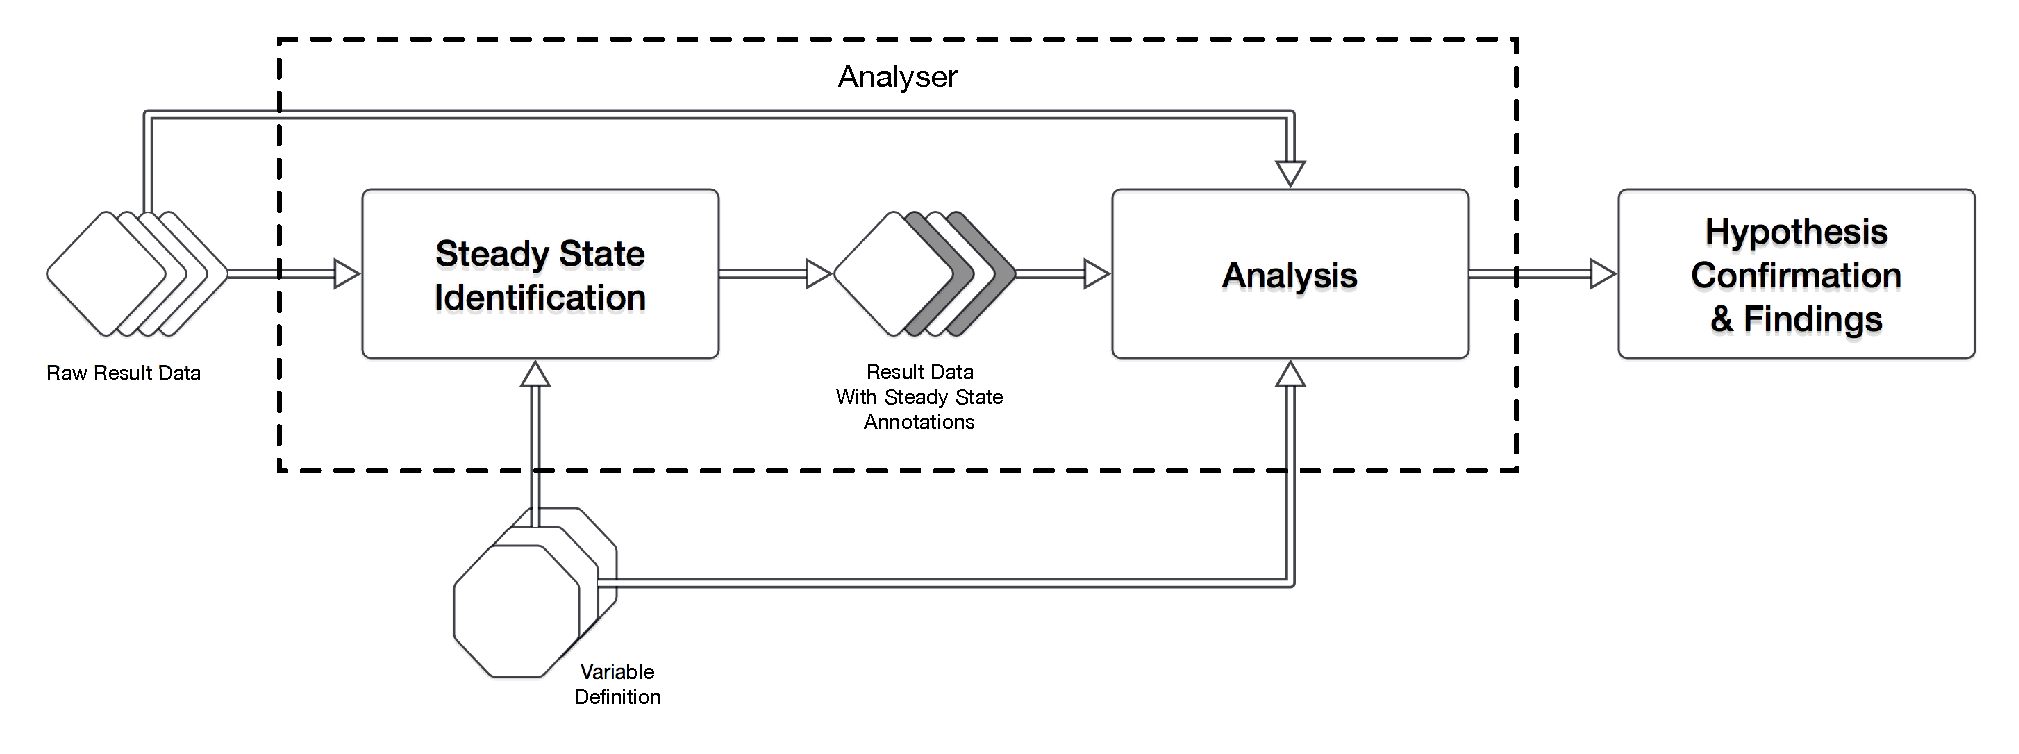
\includegraphics[width=\linewidth]{images/analyser-block-schema}
	\caption{\textsc{Analyser} Block Schema} 
  	\label{fig:analyser-block-schema}
\end{figure}

Figure \ref{fig:analyser-block-schema} shows the different phases of the data processing. The methods that compose the \textsc{Analyser} can be divided into three main block, each one with different supporting tools and different goals.

\textsc{Analyser} takes as input the raw data produced by the \textsc{Test Stand} by executing the experiment, and the variables on which the analysis will be based on. The \textsc{Test Stand} outputs raw data are in times series format and which data it outputs depend on the users needs. The \textsc{Test Stand} measurement set may variate according to the requirement [R.7]. To this extent the \textsc{Analyser} should be extendible too, and the variables of the analysis must be seen as an input provided by \name user.

To properly compare results between $n$ different RSP Engines data must be standardized. In the \textit{Steady State Identification} Block data are processed according to the variables, identifying which variable has reached a Steady State condition.

The last step in the high level Analyser Block Schema consists in the formalisation of theoretical results. The aim of this step is obviously confirm or refute hypothesis formulated at experiment design level. However, \name has the aim of sustaining the empirical research over RSP Engine which allow a new kind of observation that may improve existing theoretical models of the Stream Reasoning area.

In the next subsection we provided further details on the \textit{Steady State Identification} Block, Subsection \ref{sec:analyser-ss-block}, and about the \textit{Analysis} Block, Subsection \ref{sec:analyser-analysis-block}. The Theoretical Result Block it is not described because it depends on \name user and can not be formalised yet.

\subsection{Steady State Identification Block}\label{sec:analyser-ss-block}

\begin{figure}[tbh]
  \centering
	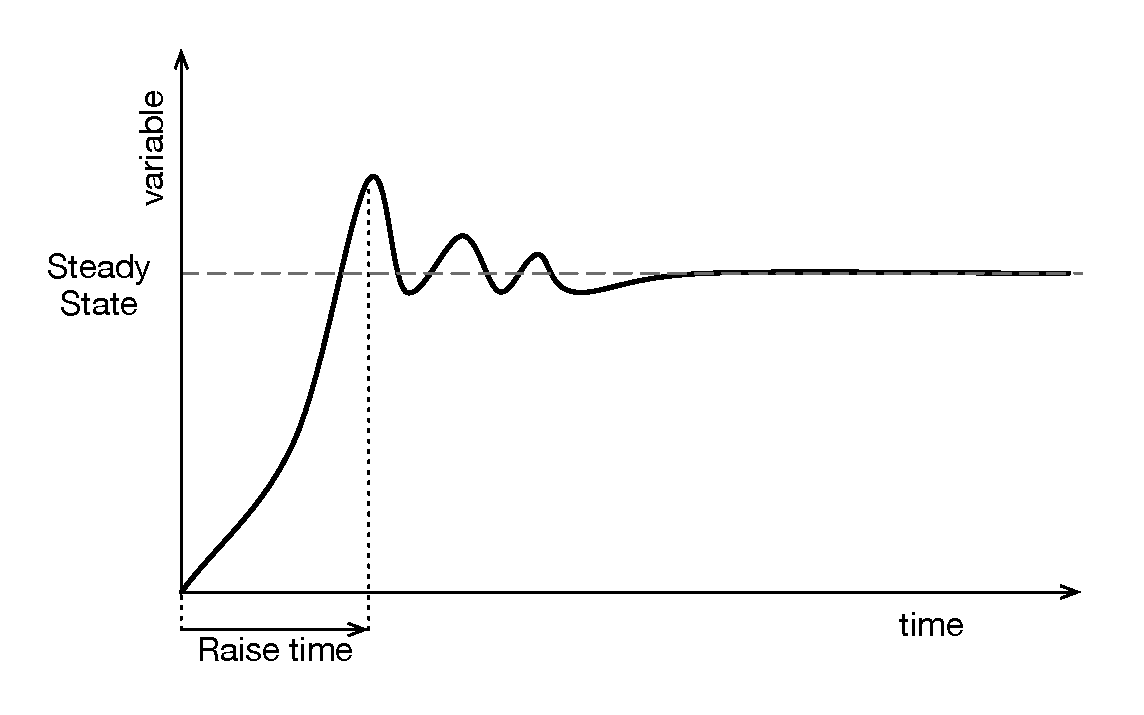
\includegraphics[width=0.5\linewidth]{images/steady-state}
	\caption{Time Series Behaviour Example in Temporal Domain} 	
  	\label{fig:steady-state}
\end{figure}

The \textit{Steady State Identification} (SSI) Block is first element in Figure \ref{fig:analyser-block-schema}. In general it applies a pre-analysis of the raw data. It outputs if a given variable of the tested RSP Engine has not reached the Steady State condition , which is the moment when a dynamic system reaches the equilibrium for a certain variable. The SSI is a common passage in almost any research on dynamic system, because those systems usually have an initial transitory phase which inhibits generalisation and comparisons. Figure \ref{fig:steady-state} shows the typical behaviour in the time domain for a certain variable and also evidences the point when the series reaches the Steady State condition. The \textit{Steady State Identification} Block allows to understand the degree of reliability of the data, how we can assume a certain observation is confirmed and generalizable. % 


\subsection{Analysis Block}\label{sec:analyser-analysis-block}

Once the Steady State is identified, it is possible to proceed with the central data analysis, which is summarised in Figure \ref{fig:analyser-block-schema} by the \textit{Analysis} Block. This Block exploits the \textit{Steady State Identification} output to study the transitory phase, which is a crucial part of the dynamic system comprehension and thus of the Hypothesis confirmation.

The investigation can be decomposed in four levels within the \textit{Analysis} Block, with increasing details degree and different goals.  Figure \ref{fig:analysis-method} is a graphical representation of the investigation stack implemented within the \textit{Analysis} Block, the detail level grows from the top to the bottom.

Before presenting the stack level one by one, we introduce two concepts about the experiment analysis:
\begin{itemize}
\item \textit{Intra Experiment Comparison} -  it means building comparisons between variables upon a single, well-determined experiment $,<\mathcal{E},<\mathcal{D},<\mathcal{T},<\mathcal{Q}>$.
\item \textit{Inter Experiment Comparison} -  it means building comparisons of different experiment 
$,<\mathcal{E},<\mathcal{D},<\mathcal{T},<\mathcal{Q}>$ and $,<\mathcal{E}',<\mathcal{D}',<\mathcal{T}',<\mathcal{Q}'>$ upon a single variable. Usually, the compared experiment differs at most for one or two elements in the tuple. 
\end{itemize}


\subsubsection{Level 0 - Dashboards}\label{sec:heaven-level0}

Dashboards are the highest level of analysis offered by \name for \textit{Inter-Experiment} comparison. Some statistical values like average (or maximum, minimum, median ecc) are presented in a n-dimension radar plot, as the one in Figure \ref{fig:radar}, which involves all the variables selected during the experiment design phase. Visual comparison of the data trough dashboards is natural when few variable are involved. It is easy to compare many solutions and identify which one is the best. The aim of dashboard is to compare experiments and pointing out the relation that occurs among the involved variables.

\begin{figure}[tbh]
  \centering
	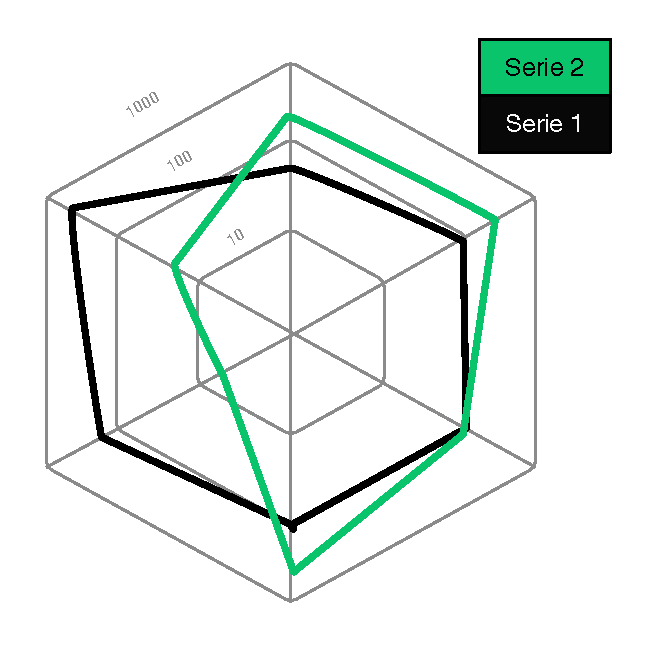
\includegraphics[width=0.5\linewidth]{images/radar-plot}
	\caption{Dashboard Example - Radar Plot} 	
  	\label{fig:radar}
\end{figure}

The idea of a single visualisation method which allows to answer to any hypothesis is desirable, but not probable.  Unfortunately, the reliability of the methods depend on the system complexity and not only on the complexity of the method itself. Thus, this level of analysis may not be able to represent the entire system complexity. The Steady State condition represents another point of weakness. If it is not reached by all the variable involved, the analysis generalisation can not be granted and dashboard relevance becomes frail. Further levels of analysis are required, at least for a better comprehension of those unpredictable results that refute even naive hypothesis, formulated on well known theoretical truths.


\subsubsection{Level 1 -  Statistical Values Comparison}\label{sec:heaven-level1}

This Analysis level focuses on a single variable at time (Latency, Memory ecc.), in a certain statistical condition (Maximum, Minimum, Mean Value ecc.) exploiting \textit{Inter-Experiment} comparison. 

To verify an hypothesis researches design and execute multiple experiments which variates for few parameters. This analysis is focused on the entries experiment set. The experiments must be arranged into an smart layout that highlights the differences between experiments upon one or more well-defined characteristics. The analysis involves one variable at time, comparing the results over the experiment set. 

The aim of Level 1 is identifying which parameter, if any, determines behaviour of the solution w.r.t the observed variable. \name enables two possible analysis approaches within Level 1:
\begin{itemize}
\item \textit{Quantitative} -  The comparison results are present in percentage form, quantifying how much a solution is better than another one under some conditions. 
\item \textit{Qualitative} - it is a simplification of the Quantitative approach. Sometimes we only need to understand which solution is the best, without focusing on numeric values. The Qualitative approach requires the definition of a tolerance threshold, for example 5\%, to distinguish when a solution is better, worse or equal to another one.
\end{itemize}

\subsubsection{Level 2 - Patter Identification}\label{sec:heaven-level2}

The comparison of a single statistical value over multiple variable (Level 0) or a single one (Level 1) may be not sufficient to explicit the RSP Engine behaviour. Starting from Level 2, visual analysis for \textit{Inter-Experiment} comparison is introduced. As in Level 1 the investigation involves a single variable over the entire experiment set, disposed into an easy-to-ready layout which points out experiment differences. Level 2 instead enables the comparison of the experiment set, presenting result data in a graphical way, which shows the system behaviour over all the experiment execution.

The aim of this level is evidencing if a certain variable a some patterns among the experiment set. How to choose the correct graphical representation depends on the variable nature and requires specific analysis. However, the most common ones for time-series are time domain form, value distribution or frequency domain representations. In general Level 2 allows to visualise how the system behaves, which is not visible with a mere model investigation.

\subsubsection{Level 3 - Visual Comparison}\label{sec:heaven-level3}

The Level 3 is the bottom level of the investigation stack. It focuses on a single solution at time and it exploits both \textit{Inter-Experiment} comparison, with the aim to understand how different experiment execution are related or to  \textit{Intra-Experiment} comparison, with the goal of pointing out the relation between the variables over all the experiment. In the first case, Level 3 reproduces the Dashboard idea but over all the experiment execution. In the second case instead, it extends what done in Level 1 and 2, but focusing on a single visualisation at time.

\begin{figure}[htb]
  \centering
	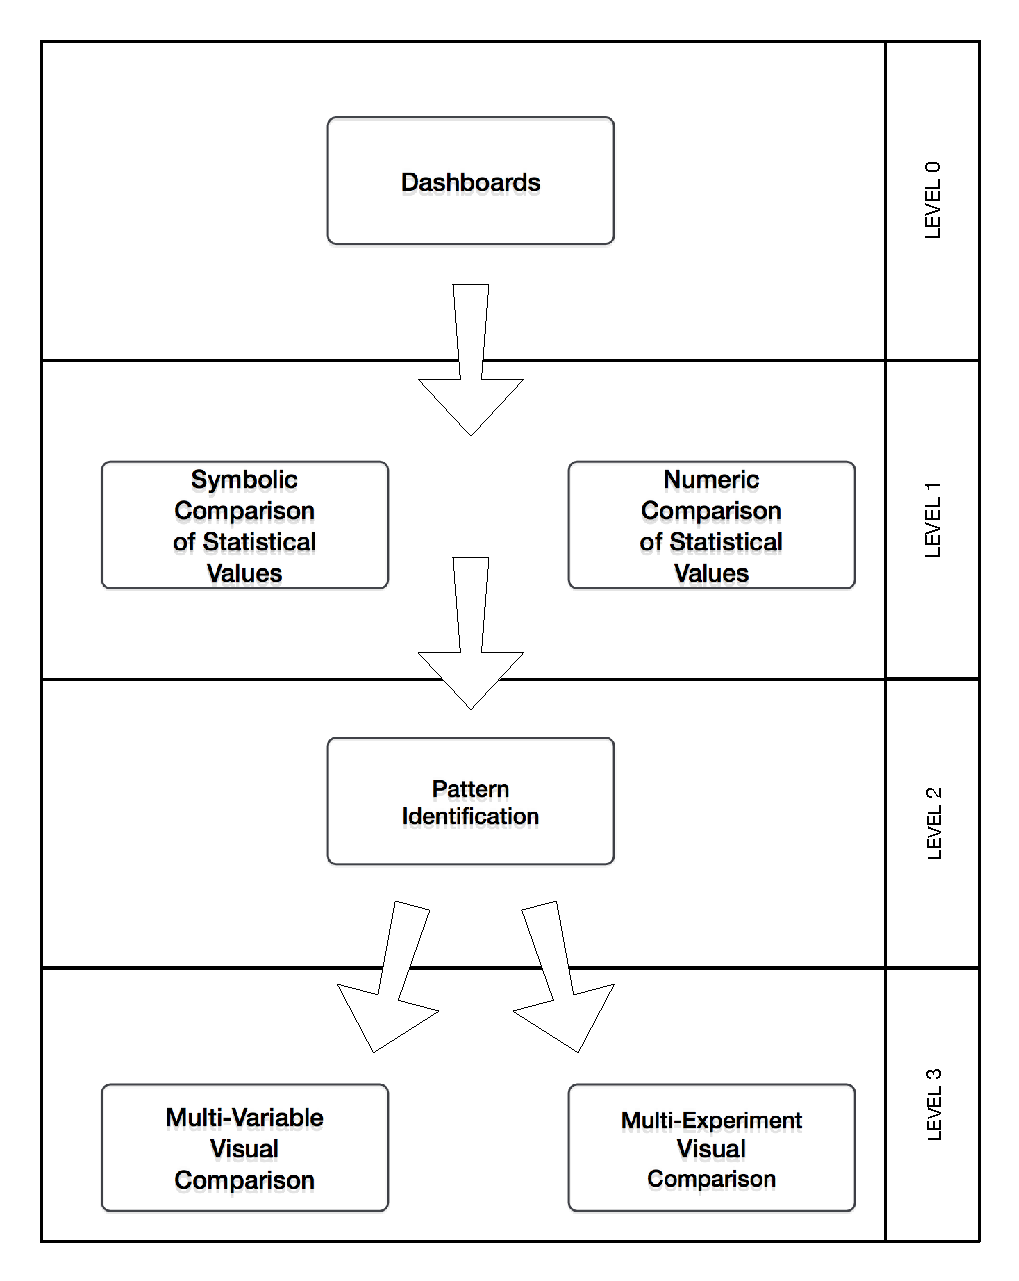
\includegraphics[width=\linewidth]{images/analysis-method}
	\caption{\textsc{Analyser} Investigation Stack}
  	\label{fig:analysis-method}
\end{figure}





%--------------------------------------------------------------------------------
% conclusions and future works
%--------------------------------------------------------------------------------
\chapter{Conclusions and Future Works}
\label{chap:conclusions}
This thesis work we presented \name -- an open source framework for empirical evaluation of RSP Engines. \name contains a Test Stand, four baselines, and an Analyser to enable the Systematic Comparative Approach in the Stream Reasoning research field

In Chapter \ref{chap:problem-settings} we present the motivation behind this work. In Chapter \ref{chap:heaven} we describe \name design and in Chapter \ref{chap:implementation-experience} we details the implementation of the Test Stand, the baselines and the investigation methods which compose the Analyser.

Finally, we provide an proof of \name potential, comparing the four baseline implementations of RSP engines with two experimental sets. The results presented in this section actually  go beyond the verification of simple hypothesis formulated on the knowledge of the RSP Engine model. We learn that, even when RSP engine is extremely simple (e.g., the baselines), it is hard to formulate  hypothesis about its behaviour and thus empirical evaluation are required. This emphasises the importance to be able to conduct comparative research based on controlled experimental conditions and, thus, the need for a open source\footnote{\url{https://github.com/streamreasoning/HeavenTeststand}} framework like \namens.

The focus on the experimental infrastructure is the main difference between \name and previous work. While SRbench and LSbench focus on RDF streams and a suite of continuous SPARQL query, \name focus on the possibility to compare RSP engines based on any RDF stream, ontology, continuous query and entailment regime. It even enables to run experiments connecting to live data streams as those used in \cite{DBLP:conf/semweb/BalduiniVDTPC13}.



\section{Research Question}

Stream Processing research field is growing and the number of techniques to semantically handle data stream is increasing. RDF Stream Processing Engines, a.k.a. RSP Engines, are system able to answer continuous extensions of SPARQL queries over RDF Streams. Due to their complexity, a systematic comparison of such systems, under repeatable conditions, is hard. It is worth to note that the lacks of a Systematic Comparative Research Approach (SCRA) belongs to entire Computer Science community, despite the Engineering epistemology of the works it publishes. This approach is typical of those research areas which have to faces very complex systems, and have difficulty to simplifies the models. Architectural analysis are useful, but they are not sufficient to complete evaluate RSP Engine, because their behaviour must be studied during the execution. For this reason, the Stream Reasoning community has tried to define and develop solution to evaluate RSP Engines. Recent works supported the SCRA on RSP Engines with queries, dataset and methods. However the SR community still lacks an experimental infrastructure which enables the comparison of RSP Engines based on any RDF stream, ontology, continuous query and entailment regime.  For me aerospace engineering we borrow the idea of engine test stand: a facility to develop engine trough systematic testing under precise experimental conditions. Thus, we can formulate our research question as follows:

”Can an engine test stand, together with queries, datasets and methods, support SCRA for Stream Reasoning?”


\section{Results}
\section{Limitations}
\section{Future Works}

Our future works can focus on the different parts of \name. Our main interest is benchmarking existing time-based sliding window RSP engines. To this end, we intend to extend the \textsc{Flow Rate Profiler} in order to generate: a random flow with a given distribution (e.g., gaussian and exponential), and a sine wave flow (to mimic the periodic changes in the flow rates observed on social media streams \cite{DBLP:conf/semweb/BalduiniVDTPC13}). We also intend to add the possibility to register one or more continuous queries into the baselines\footnote{In the current stage of development it is possible to configure the ontology and the entailment regime.}. Offering \name as a service is our long term goal. 

We are imagining  this as a Web-based environment where all existing RSP engines are already available and those, who want to run experiments, have just to configure them picking up one or more RDF streams, ontologies, and queries. A visual facility to compare different experiments and the publication of result experiments as linked data would complete this environment.


%--------------------------------------------------------------------------------
% appendices
%--------------------------------------------------------------------------------
\part*{Appendices\label{part:app}\addcontentsline{toc}{part}{Appendices}}
\appendix
\chapter{\dots}
\label{app:one}
\section{Introduction}
Introduzione agli argomenti trattati nell'appendice, dalle 4 alle 10 righe.

\section{\dots}
Argomenti trattati suddivisi sezione per sezione. 
Alla fine del capitolo non includere alcun sommario.



\chapter{\dots}
\label{app:two}
\section{Introduction}
Introduzione agli argomenti trattati nell'appendice, dalle 4 alle 10 righe.

\section{\dots}
Argomenti trattati suddivisi sezione per sezione. 
Alla fine del capitolo non includere alcun sommario.


\bibliographystyle{plain}
\bibliography{tesi.bib}
\end{document}
